\documentclass[10pt]{beamer}
\usepackage{amsmath}
\usepackage{mathtools}
\usepackage{multimedia}
\usepackage{hyperref}


\usefonttheme{professionalfonts} % using non standard fonts for beamer
\usefonttheme{serif} % default family is serif
%\documentclass[12pt]{beamerthemeSam.sty}
\usepackage{epsf}
%\usepackage{pstricks}
%\usepackage[orientation=portrait,size=A4]{beamerposter}
\geometry{paperwidth=160mm,paperheight=120mm}
%DT favorite definitions
\def\LL{\left\langle}	% left angle bracket
\def\RR{\right\rangle}	% right angle bracket
\def\LP{\left(}		% left parenthesis
\def\RP{\right)}	% right parenthesis
\def\LB{\left\{}	% left curly bracket
\def\RB{\right\}}	% right curly bracket
\def\PAR#1#2{ {{\partial #1}\over{\partial #2}} }
\def\PARTWO#1#2{ {{\partial^2 #1}\over{\partial #2}^2} }
\def\PARTWOMIX#1#2#3{ {{\partial^2 #1}\over{\partial #2 \partial #3}} }

\def\rightpartial{{\overrightarrow\partial}}
\def\leftpartial{{\overleftarrow\partial}}
\def\diffpartial{\buildrel\leftrightarrow\over\partial}

\def\BS{\bigskip}
\def\BC{\begin{center}}
\def\EC{\end{center}}
\def\BN{\begin{enumerate}}
\def\EN{\end{enumerate}}
\def\BI{\begin{itemize}}
\def\EI{\end{itemize}}
\def\BE{\begin{displaymath}}
\def\EE{\end{displaymath}}
\def\BEA{\begin{eqnarray*}}
\def\EEA{\end{eqnarray*}}
\def\BNEA{\begin{eqnarray}}
\def\ENEA{\end{eqnarray}}
\def\EL{\nonumber\\}

\newcommand{\etal}{{\it et al.}}
\newcommand{\gbeta}{6/g^2}
\newcommand{\la}[1]{\label{#1}}
\newcommand{\ie}{{\em i.e.\ }}
\newcommand{\eg}{{\em e.\,g.\ }}
\newcommand{\cf}{cf.\ }
\newcommand{\etc}{etc.\ }
\newcommand{\atantwo}{{\rm atan2}}
\newcommand{\Tr}{{\rm Tr}}
\newcommand{\dt}{\Delta t}
\newcommand{\op}{{\cal O}}
\newcommand{\msbar}{{\overline{\rm MS}}}
\def\chpt{\raise0.4ex\hbox{$\chi$}PT}
\def\schpt{S\raise0.4ex\hbox{$\chi$}PT}
\def\MeV{{\rm Me\!V}}
\def\GeV{{\rm Ge\!V}}

%AB: my color definitions
%\definecolor{mygarnet}{rgb}{0.445,0.184,0.215}
%\definecolor{mygold}{rgb}{0.848,0.848,0.098}
%\definecolor{myg2g}{rgb}{0.647,0.316,0.157}
\definecolor{A}{rgb}{1.0,0.3,0.3}
\definecolor{B}{rgb}{0.0,1.0,0.0}
\definecolor{C}{rgb}{1.0,1.0,0.0}
\definecolor{D}{rgb}{0.5,0.5,1.0}
\definecolor{E}{rgb}{0.7,0.7,0.7}
\definecolor{abtitlecolor}{rgb}{1.0,1.0,1.0}
\definecolor{absecondarycolor}{rgb}{0.0,0.416,0.804}
\definecolor{abprimarycolor}{rgb}{1.0,0.686,0.0}
\definecolor{Red}           {rgb}{1,0.4,0.4}
\definecolor{Yellow}           {rgb}{1,1,0.0}
\definecolor{Grey}          {cmyk}{.7,.7,.7,0}
\definecolor{Blue}          {cmyk}{1,1,0,0}
\definecolor{Green}         {cmyk}{1,0,1,0}
\definecolor{Brown}         {cmyk}{0,0.81,1,0.60}
\definecolor{Silver}        {rgb}{0.95,0.9,1.0}
\definecolor{Sky}           {rgb}{0.07,0.0,0.2}
\definecolor{Darkbrown}     {rgb}{0.4,0.3,0.2}
\definecolor{40Gray}        {rgb}{0.4,0.4,0.5}
\usetheme{Madrid}


\setbeamercolor{normal text}{fg=Silver,bg=Sky}

%AB: redefinition of beamer colors
%\setbeamercolor{palette tertiary}{fg=white,bg=mygarnet}
%\setbeamercolor{palette secondary}{fg=white,bg=myg2g}
%\setbeamercolor{palette primary}{fg=black,bg=mygold}
\setbeamercolor{title}{fg=abtitlecolor}
\setbeamercolor{frametitle}{fg=abtitlecolor}
\setbeamercolor{palette tertiary}{fg=white,bg=Darkbrown}
\setbeamercolor{palette secondary}{fg=white,bg=absecondarycolor}
\setbeamercolor{palette primary}{fg=white,bg=40Gray}
\setbeamercolor{structure}{fg=abtitlecolor}

\setbeamerfont{section in toc}{series=\bfseries}

%AB: remove navigation icons
\beamertemplatenavigationsymbolsempty
\title[Light]{
  \textbf {Light}}


\author [Astronomy 101]{Astronomy 101\\Syracuse University, Fall 2019\\Walter Freeman}

\date{\today}

\begin{document}

\frame{\titlepage}
\frame{
\BC
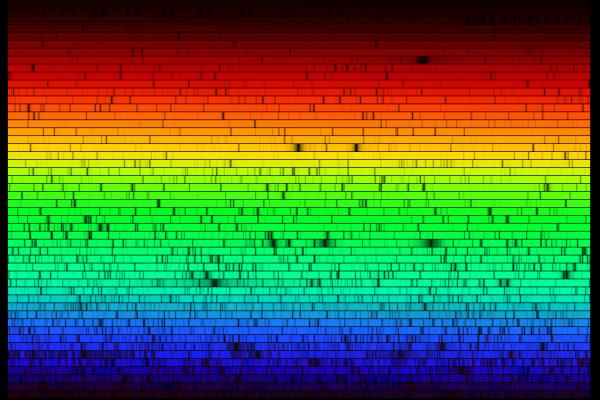
\includegraphics[width=0.9\textwidth]{solarspectrum.jpg}
\large

This is a ``picture'' of the Sun. What can we learn from it?
\EC
}

\frame{\frametitle{\textbf{Announcements}}

\Large

\BI
\item I'm catching up after being out sick for a while
\item I am way behind on answering email and messages because of this
\item The Scantron folks closed early on Friday because of sportsball and I was out sick Monday
\item You should have your Exam 2 grades late tomorrow
\item I'll post an answer key with the exam tomorrow as well
\EI
}

\frame{\frametitle{\textbf{Paper 2}}
	\Large
	\BI
	\item Paper 2's assignment is posted
	\item It is due three weeks from tomorrow.
	\pause
	\bigskip
	\item This paper is an argumentative paper:
	\BI
	\large
	\item You're telling us that someone else is wrong
	\item You can be bold in making these claims, as long as you argue your point well!
	\EI
	\EI
}

\frame{

\large
\BC
How much of the light in this room can you see?\EC

\BS\BS
\Large
\color{A}A: All of it\\
\color{B}B: Most of it \\
\color{C}C: Around a quarter of it\\
\color{D}D: Not much of it at all\\
}

\frame{
\large
\BC
\large
How much of the sound in this room can you hear?\EC
\Large
\BS\BS

\color{A}A: All of it\\
\color{B}B: Most of it \\
\color{C}C: Around a quarter of it\\
\color{D}D: Not much of it at all\\
}

\frame{
\large
\BC
Sounds can have a spectrum of frequencies and wavelengths, 
and we can only perceive a piece of that spectrum.

\BS\BS\pause

\BS

In the same way {\it light} has a spectrum of frequencies/wavelengths, 
and our eyes only perceive a tiny fraction of that spectrum.

\color{Red}
When we say ``light'', we mean {\it all} wavelengths, not just the 
ones we can see!
\EC
}

\frame{\frametitle{\bf The electromagnetic spectrum}

\BC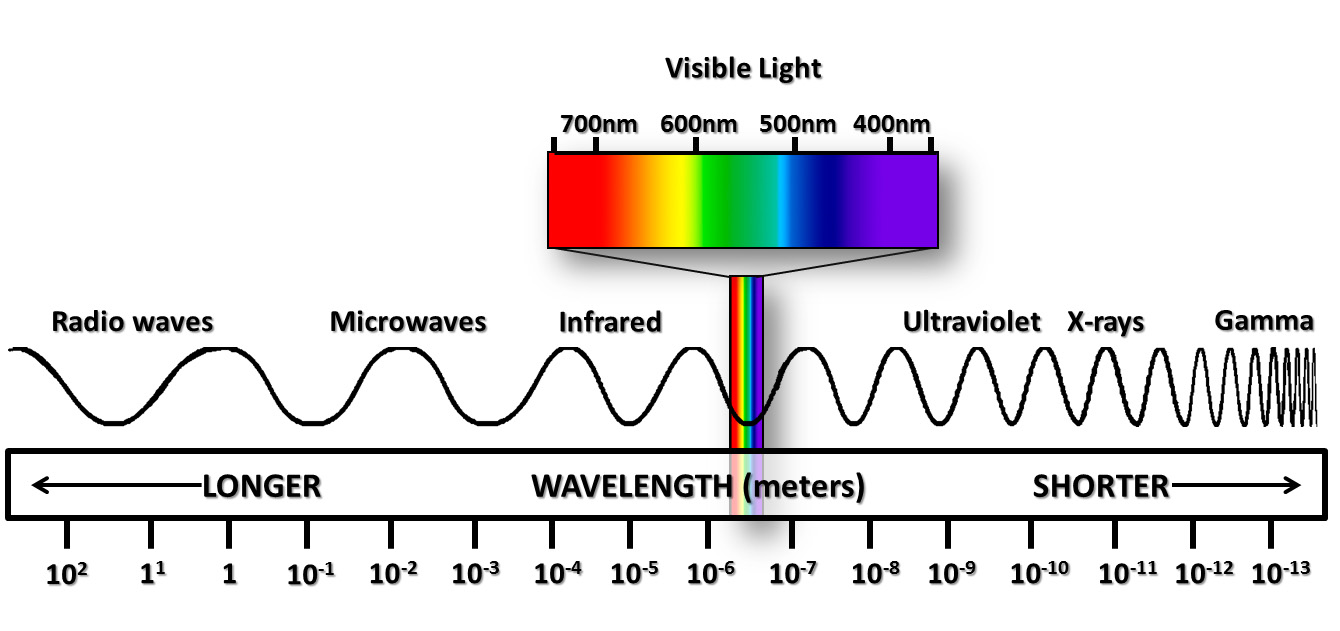
\includegraphics[width=0.8\textwidth]{linear-spectrum.jpg}

\BS

There is an enormous range of ``colors'' of light out there!\EC

\BS\BS

What's this ``sound'' like?

\pause
\BS
{Music: ``The Blood of Cu Chulainn'', from the soundtrack to {\it Boondock Saints} (Jeff Danna, 1999)}

\BS\pause

We can learn far more about what's going on in the orchestra if we 
have the whole spectrum, rather than just a piece!
}

\frame{
\BC
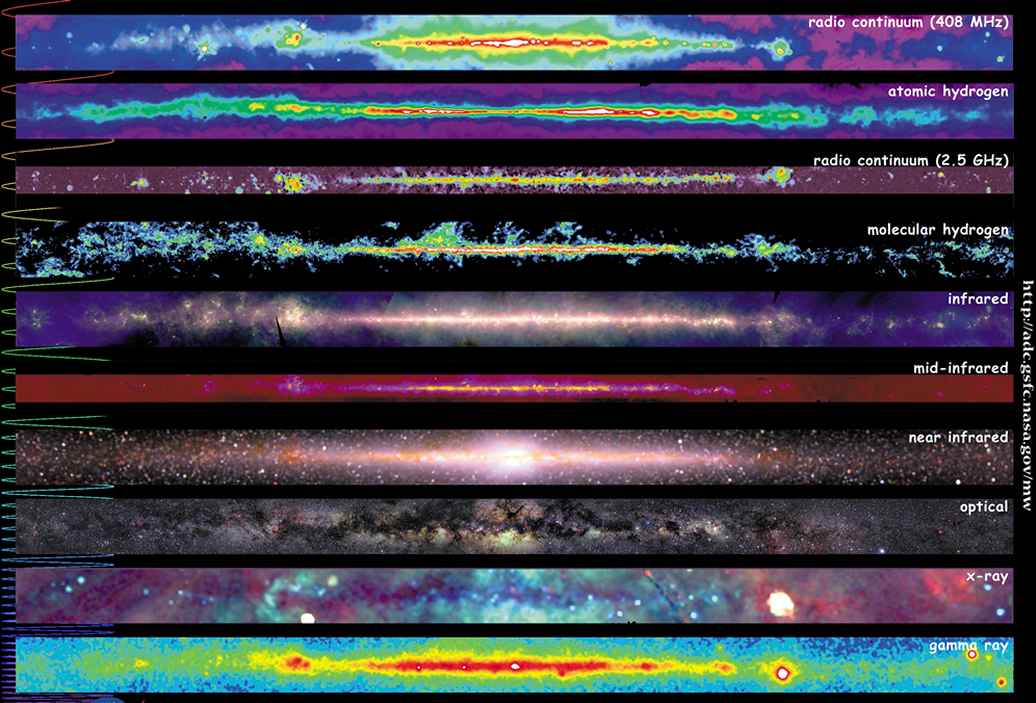
\includegraphics[height=0.9\textheight]{mwmw.jpg}
\EC
}



\frame{\frametitle{\bf{An illuminating story}}

In the late 19th century, the laws of electromagnetism looked like this:

\BI
\item Electric fields exert a force on electric charges
\item Magnetic fields exert a force on {\it moving} electric charges
\EI

\bigskip

We know this thanks in large part to the work of Michael Faraday, who
famously wasn't good at algebra and drew pictures of fields.

\bigskip

Where do these fields come from?

\BI
\item Electric charges make electric fields
\item Moving electric charges make magnetic fields
\item Changing magnetic fields make electric fields
\pause
\item {\color{Red} Changing electric fields make magnetic fields}
\EI
}

\frame{\frametitle{\bf{An illuminating story}}

\begin{columns}
\column{0.6\textwidth}
\BI
\item Electric charges make electric fields
\item Moving electric charges make magnetic fields
\item Changing magnetic fields make electric fields
\item {\color{Red} Changing electric fields make magnetic fields}
\EI

\BS

Last law added by James Clerk Maxwell in the 1860's, and it has
a surprising consequence:

\BS
\BI
\item{Changing electric field makes a magnetic field}
\pause \item ... which makes a magnetic field ...
\pause \item ... which makes an electric field further away ...
\pause \item This leads to a traveling electromagnetic disturbance: an {\it electromagnetic wave}.
\EI
\column{0.4\textwidth}
\begin{center}
	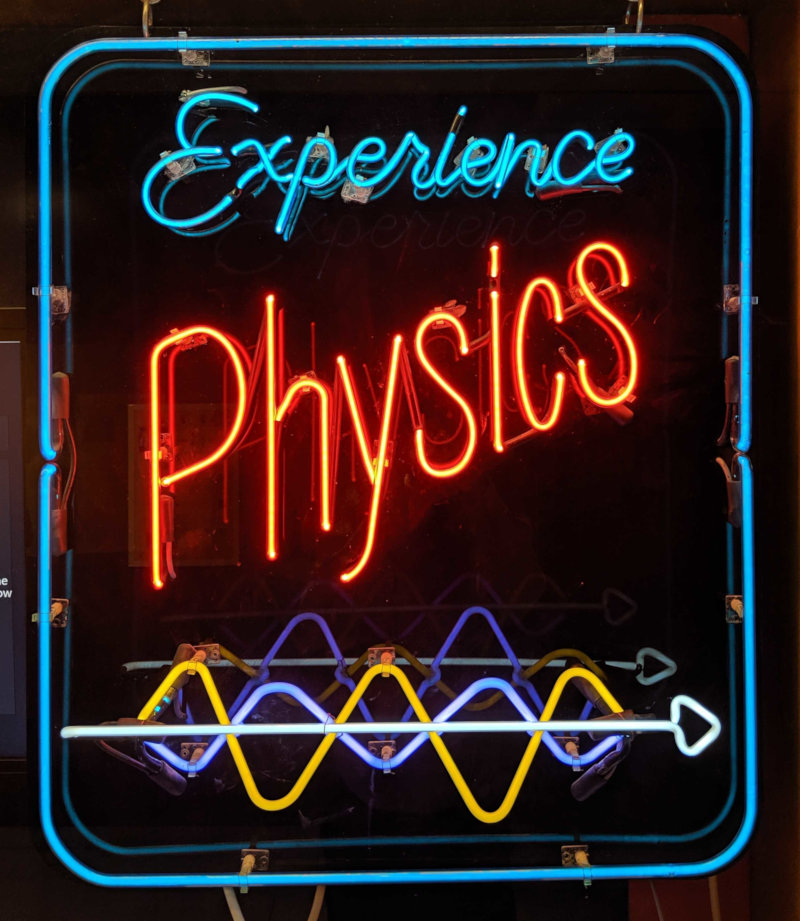
\includegraphics[width=0.95\textwidth]{experiencephysics.jpg}
	\end{center}
\end{columns}
}

\frame{\frametitle{\bf{An illuminating story}}

Maxwell calculated that these electromagnetic waves traveled at
around 300 million meters per second.

\BS

Independently, light had been measured to travel at 300 million
meters per second some years prior.

\BS \pause

So ... if this electromagnetic wave travels at the speed of
light, perhaps it {\it is} light?

\BS

In the history of science, sometimes theory gets ahead of experiment -- like in the discovery of the nature of light.
}

\frame{\frametitle{\bf{The properties of waves}}
\Large

\BC
Light is a traveling {\it electromagnetic wave}. This means:
\EC

\BS
\large

\BI
\item ... it moves through space at some {\color{Red}speed: the speed of light, $c=3 \times 10^8$ m/s.}
\pause\BS
\item ... these waves have a {\color{Yellow}wavelength}: the distance from peak to peak of the electric field. We use the letter {\color{Yellow}$\lambda$} for wavelength.
\pause\BS
\item ... and, as an observer holds still, a certain number of waves pass that observer per second. This is called the {\color{Green}frequency, $f$}.
\EI

\BC 
\Large How are these things related? Let's look at a simulation...
\EC
}

\frame{

\Large

Three basic wave properties:

\BI
\item \color{Red}Wave speed: $c$
\item \color{Yellow}Wavelength: $\lambda$
\item \color{Green}Frequency: $f$
\EI

\BS\BS

If I keep {\color{Red}$c$} constant and increase {\color{Yellow}$f$}, then {\color{Green}$\lambda$} will \underline{\hspace{3cm}}...

\BS\BS
If I keep {\color{Red}$c$} constant and decrease {\color{Yellow}$f$}, then {\color{Green}$\lambda$} will \underline{\hspace{3cm}}...

\BS\BS

If I keep {\color{Green}$\lambda$} constant and increase {\color{Red}$c$}, then {\color{Yellow}$f$} will \underline{\hspace{3cm}}...
}

\frame{
\Large
\BC
This leads us to the basic relation:
\Huge $$\color{Red}c = \color{Yellow}f \color{Green}\lambda$$
\large
Or in words:
\huge
$$
{\color{Red}(\text {speed of light})} = {\color{Yellow}(\text{frequency})} \times {\color{Green}(\text{wavelength})}
$$

\large

This is easy to remember by thinking about how each quantity is measured:
\huge
$$
{\color{Red}\frac{\text {meters}}{\text{second}}} = {\color{Yellow}\frac{\text{waves}}{\text{second}} }\times {\color{Green}\frac{\text{meters}}{\text{wave}}}
$$

\EC



This means:
\large
\BI
\item Shorter wavelengths have higher frequency
\item Longer wavelengths have lower frequency
\EI

}

\frame{
\Large

Newton wrote about light, and thought that it came in little chunks called {\it corpuscles} that flew through space in
straight lines, like bullets.

\BS

Maxwell deduced that it was a {\color{Red}wave}, and experiments confirmed that.

\BS\BS\pause
You should know:

\BI
\item Energy per photon is {\it proportional} to the frequency of the light
\item Energy per photon is {\it inversely proportional} to its wavelength
\item Wavelength is inversely proportional to frequency
\EI
... but later experiments (which we'll see soon) showed that it had to come in discrete chunks! What gives?

\BS

Is light a wave, or is it a bunch of little {\color{Green}particles?}

\BS\BS

It turns out that, in quantum mechanics, it can be {\it both}, and everyone gets to be right!

}

\frame{\frametitle{\textbf{The quantum nature of light}}

Light has both particle properties and wave properties:

\BI
\item Particle properties: it comes in discrete chunks called {\it photons}, each carrying a certain {\color{Green}energy}.
\item Wave properties: it has a {\color{Red} wavelength} $\lambda$ and {\color{Red} frequency} $f$ 
\EI

It turns out that shorter-wavelength, higher-frequency light has higher energy per photon. The relationship is:

\Huge
$$E=hf=hc/\lambda$$

\large

This value $h$ is called Planck's constant. It is baked into the fabric of the Universe, like $G$ and $c$:

\bigskip
\BI
\item $G$, the universal gravitational constant: tells us how strong gravity is
\item $c$, the speed of light: tells us how fast light goes
\pause
\item \color{Red}$h$, Planck's constant: tells us how ``lumpy'' light is: how much energy do photons of a given frequency have?
\EI

}

\frame{\frametitle{\textbf{Things you should know:}}

\Large Light is both a particle and a wave.
\BS

\BI
\item All light travels at the same speed, $c = $ 300 million m/s, in vacuum
\item Light comes in little lumps called {\it photons}
\item Energy per photon is {\it proportional} to the frequency of the light
\item Energy per photon is {\it inversely proportional} to its wavelength
\item Wavelength is inversely proportional to frequency
\EI
}

\frame{

\BC
\Large
We have lots of names for different sorts of light.

\BS

They differ only in wavelength/energy/frequency, and the other things they interact with.
\EC

\large
\BI
\item Radio waves: used to communicate over long distances

\BS

\item Microwaves: used to communicate over short distances

\BS

\item ``Far infrared'': associated with objects with temperatures close to ours

\BS

\item ``Near infrared'': much like light, but we can't see it

\BS

\item Visible light (only a very narrow range!)

\BS

\item Ultraviolet: enough energy to disrupt atoms

\BS

\item X-rays: enough energy to penetrate human tissue

\BS

\item Gamma rays: enough energy to disrupt atomic nuclei!

\BS

\EI

}

\frame{

\BC
\Large All of these are ``types of light''. 

\BS

They differ only in wavelength/frequency/energy!

\BS\BS

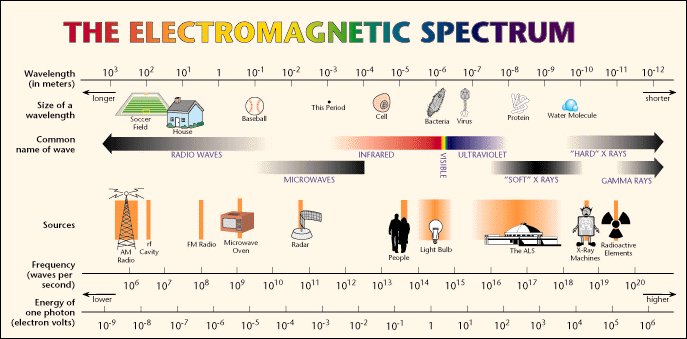
\includegraphics[width=\textwidth]{EMSpec.png}
\EC
}

\frame{
\BC
\Huge
Complete {\it Lecture Tutorials} pp. 47-49.

\normalsize

\BS\BS

We will play with some toys after this.
\EC

}

\end{document}
